% figure: ctrl-feedforward-block.png
% 用途：自控 03-8-1 扰动误差与前馈补偿原理 —— 按输入前馈的结构
% 构建：..\build.ps1 -File .\block-feedforward.tex
% 说明：① 旧图纵向太扁（980x360），且标签非数学体；
%       ② 旧图把前馈标作 G_c(s)，与笔记正文口径不符（正文说"图中的顺馈 G_c 在本篇
%          记作 F_r"），本图直接标 F_r，正文那句解释因此成为多余，已同步删去。
\documentclass[border=10pt]{standalone}
\usepackage{fontspec}
\setmainfont{Cambria}
\usepackage{unicode-math}
\setmathfont{Cambria Math}
\usepackage{tikz}
\usetikzlibrary{positioning, arrows.meta, calc}
\usepackage{ctex}

\definecolor{figink}{HTML}{1E2228}
\definecolor{figacc}{HTML}{B23020}
\definecolor{figsub}{HTML}{606874}
\definecolor{figfill}{HTML}{E8EFF8}

\begin{document}
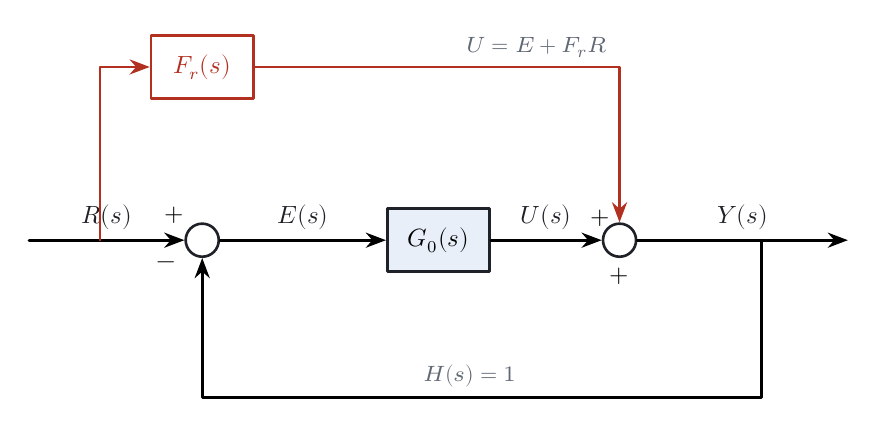
\begin{tikzpicture}[
  x=1cm, y=1cm,
  line width=0.95pt, line cap=round, line join=round,
  >=Stealth,
  blk/.style = {draw=figink, line width=0.95pt, fill=figfill,
                minimum width=1.3cm, minimum height=0.8cm, inner sep=2pt,
                anchor=center, font=\small},
  blkacc/.style = {draw=figacc, line width=0.95pt, fill=white,
                minimum width=1.3cm, minimum height=0.8cm, inner sep=2pt,
                anchor=center, font=\small, text=figacc},
  sum/.style = {draw=figink, line width=0.95pt, circle, inner sep=0pt,
                minimum size=0.42cm, anchor=center},
  sig/.style = {font=\small, color=figink},
  acc/.style = {font=\small, color=figacc},
  lbl/.style = {font=\small, inner sep=1.5pt},
  sub/.style = {font=\footnotesize, color=figsub}
]

\node[sum] (s1) at (0,0) {};
\node[blk] (g0) at (3.0,0) {$G_0(s)$};
\node[sum] (s2) at (5.3,0) {};
\node[blkacc] (fr) at (0,2.2) {$F_r(s)$};

% 输入
\draw[->] (-2.2,0) -- node[sig, above] {$R(s)$} (s1.west);
\draw[->] (s1.east) -- node[sig, above] {$E(s)$} (g0.west);
\draw[->] (g0.east) -- node[sig, above] {$U(s)$} (s2.west);
\draw[->] (s2.east) -- node[sig, above] {$Y(s)$} (8.2,0);

% 前馈支路：R -> F_r -> U
\draw[->, figacc] (-1.3,0) -- (-1.3,2.2) -- (fr.west);
\draw[->, figacc] (fr.east) -- (5.3,2.2) -- (s2.north);

% 单位负反馈
\draw[->] (7.1,0) -- (7.1,-2.0) -- (0,-2.0) -- (s1.south);
\node[sub] at (3.4,-1.72) {$H(s)=1$};

\node[lbl] at (-0.36,0.32) {$+$};
\node[lbl] at (-0.46,-0.32) {$-$};
\node[lbl] at (5.06,0.28) {$+$};
\node[lbl] at (5.3,-0.46) {$+$};

\node[sub] at (-1.5,1.1) {前馈};
\node[sub] at (4.0,2.45) {按输入前馈 $U=E+F_rR$};

\end{tikzpicture}
\end{document}
